\section{SCDP: Spherical Channel Density Prediction}

\begin{frame}{SCDP Architecture Overview}
    \begin{itemize}
        \item Basis-based approach with following ingredients:
        \begin{itemize}
            \item Virtual nodes for non-local electronic structures
            \item Even-tempered Gaussian basis sets
            \item High-capacity equivariant spherical channel network (eSCN).
        \end{itemize}
        \item Charge density representation with trainable scale parameters:
        \begin{align*}
            \rho(\mathbf{r}) &= \sum_a \sum_l^{N_a} \sum_{m = -l}^{l} c_{alm}
            \Phi_{\alpha,l,m,\mathbf{r}_a}(\mathbf{r}, s_{al}) \\
            \Phi_{\alpha,l,m,\mathbf{r}_i}(\mathbf{r}, s) &= 
            z_{\alpha,l,s} \exp(-s \cdot \alpha |\mathbf{r} - \mathbf{r}_a|^2) 
            |\mathbf{r} - \mathbf{r}_a|^l Y_{lm}(
                \widehat{\mathbf{r} - \mathbf{r}_a})
        \end{align*}
        \item Model prediction, scaling factors $s_{al} \in (0.5, 2.0)$:
        \begin{align*}
            \{c_{alm}, s_{al}\} &= F(\{(\mathbf{r}_a, Z_a)\}).
        \end{align*}
    \end{itemize}
\end{frame}


\begin{frame}{Virtual Nodes and Basis Sets}
    \begin{itemize}
        \item Virtual nodes:
        \begin{itemize}
            \item Placed at bond midpoints.
            \item Use oxygen basis functions
            \item SE(3)-equivariant placement
        \end{itemize}
        \item Even-tempered Gaussian basis for better accuracy:
        \begin{align*}
            \alpha_k &= \alpha \cdot \beta^k \text{ for } k = 0,1,2,...,N_l
        \end{align*}
        \item  Reducing SO(3) convolution to SO(2): $O(L^6) \rightarrow O(L^3)$.
        \item  The basis set is not orthonormal, the coefficients depend on the
        cutoff radius.
        \item Two-stage training for stability caused by the scale factors
        on the exponent:
        \begin{itemize}
            \item pre-train the model with fixed basis set exponents
            \item fine-tune the prediction model with a small learning rate with
            the learning for scaling factors enabled.
        \end{itemize}
    \end{itemize}
\end{frame}


\begin{frame}{Model Architecture}
    \begin{itemize}
        \item Backbone: eSCN (equivariant spherical channel network)
        \begin{itemize}
            \item $\{x_a\} = \text{eSCN}(\{(\mathbf{r}_a, Z_a)\})$
            \item Complexity: $O(L^3)$ vs $O(L^6)$ for tensor products
            \item Features: Multi-channel spherical harmonics
            \item Example: $128\times0e + 128\times1o + 128\times2e + 128\times3o$
        \end{itemize}
        \item Prediction layers:
        \begin{align*}
            \{c_{alm}, h_i\} &= \text{FullyConnectedTensorProduct}(x_i, x_l) \\
            s_{al} &= \frac{C_1}{1 + \exp(-\text{Linear}(h_i) + \ln C_2)} + C_3
            \in [C_1, C_3].
        \end{align*}
        \item Training objective:
        \begin{align*}
            \mathcal{L} &= \mathbb{E}_{\mathbf{r}\in\text{Data}}[|\rho(\mathbf{r}) - \hat{\rho}(\mathbf{r})|]
        \end{align*}
    \end{itemize}
\end{frame}


% \begin{frame}{pseudocode}
%     \begin{figure}
%         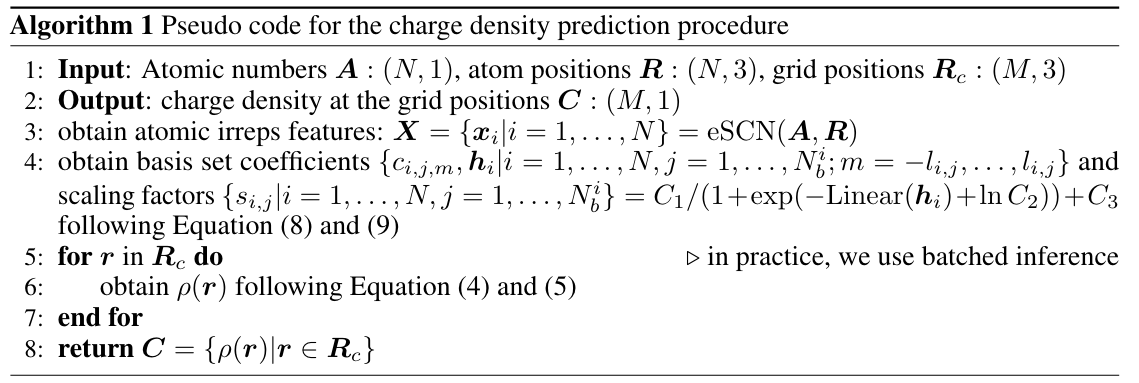
\includegraphics[width=\textwidth]{figures/scdp_3.jpg}
%     \end{figure}
% \end{frame}


\begin{frame}{Performance Analysis}
    \begin{itemize}
        \item NMAE: 0.178\% on QM9 test set
        \item 31.7x faster than ChargE3Net
        \item Flexible accuracy-efficiency trade-off
    \end{itemize}
    \begin{figure}
        \begin{subfigure}{0.48\textwidth}
        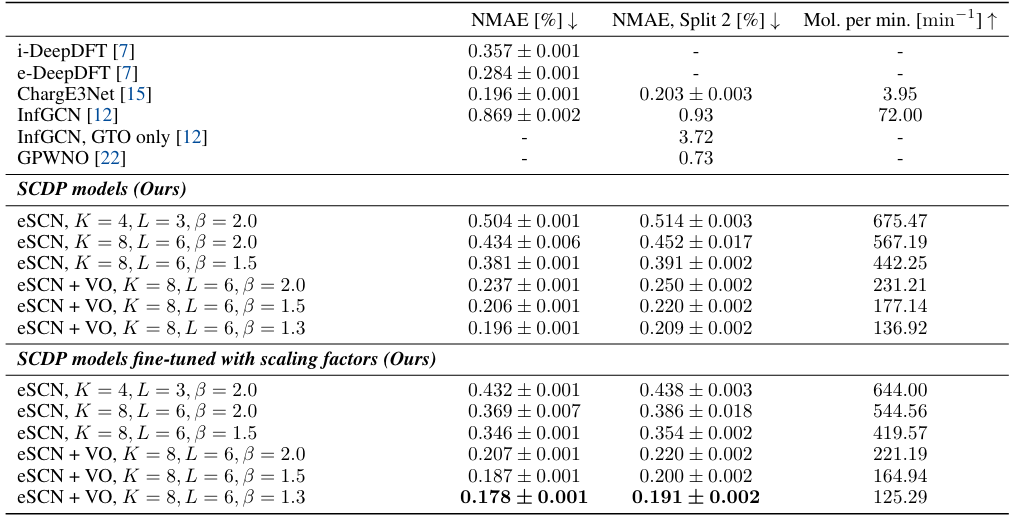
\includegraphics[width=\textwidth]{figures/scdp_2.jpg}
    \end{subfigure}
    \begin{subfigure}{0.48\textwidth}
        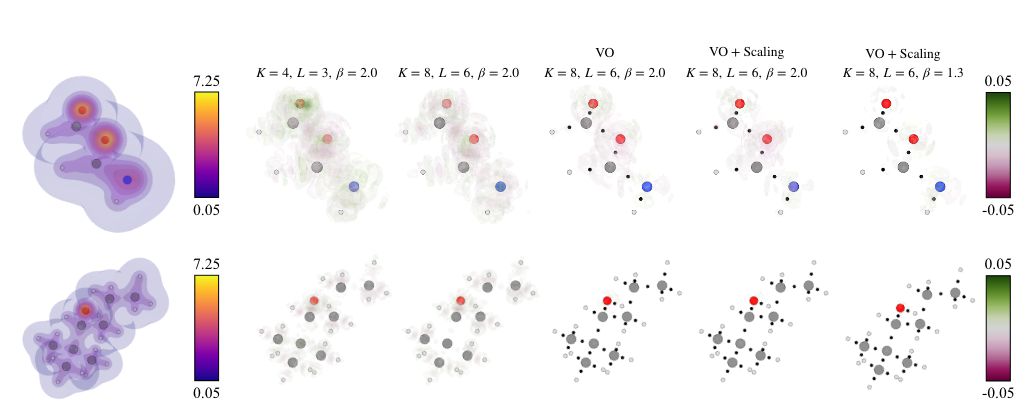
\includegraphics[width=\textwidth]{figures/scdp_1.jpg}
    \end{subfigure}
    \end{figure}
\end{frame}
